% Asset ID: A22StatisticalHypothesisTestingTIKZ-002
% Unit code: A22
% Topic code: A22-HT
% Topic name: Statistical hypothesis testing
% Related lesson section: Exam Technique, Critical regions
% Source: CCEA specification map; lesson transcript; Stats Yr2 Chapter 1 PDF
% Purpose: Show positive one-tailed, negative one-tailed and two-tailed critical regions for PMCC tests.
% Status: Phase 4 TikZ draft

\documentclass[tikz,border=8pt]{standalone}
\usepackage{amsmath}
\usepackage{tikz}
\usetikzlibrary{arrows.meta, positioning}
\begin{document}
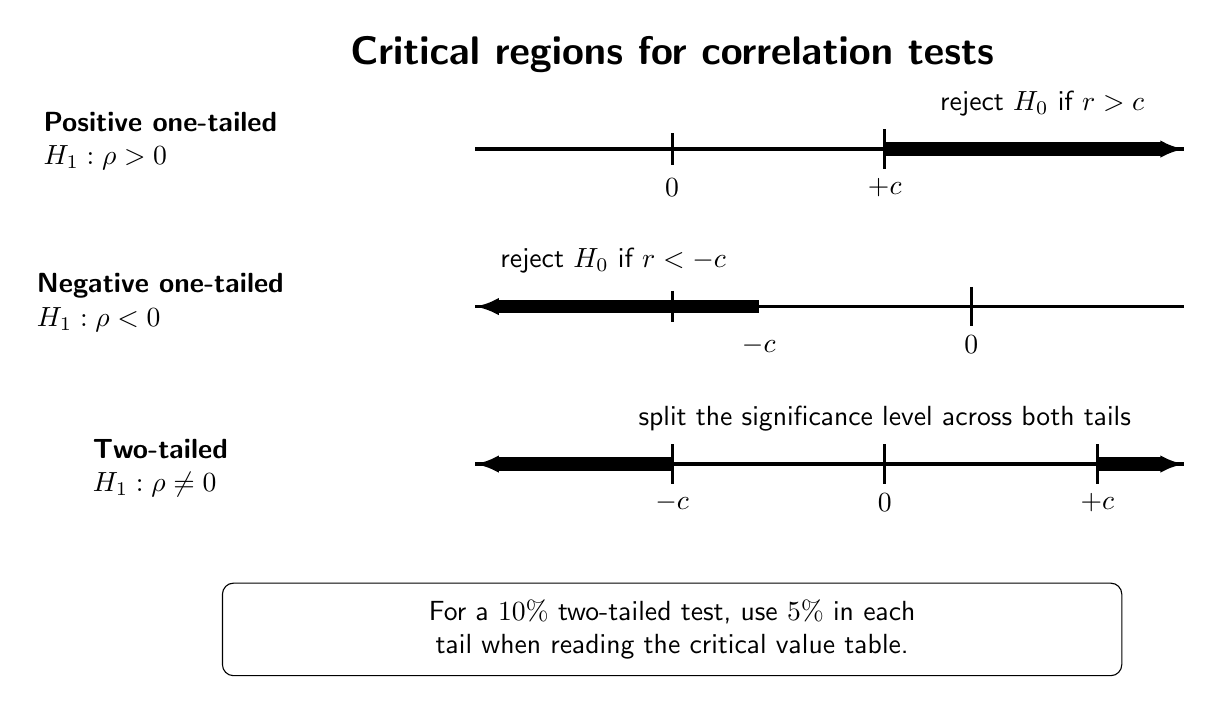
\begin{tikzpicture}[font=\sffamily, axis/.style={line width=1.2pt}, crit/.style={line width=5pt}, tick/.style={line width=1pt}, note/.style={align=left}]
\node[font=\sffamily\bfseries\Large] at (0,4.2){Critical regions for correlation tests};
\node[note] at (-6.5,3.1) {\textbf{Positive one-tailed}\\\(H_1:\rho>0\)};
\draw[axis] (-2.5,3) -- (6.5,3); \draw[tick] (2.7,3.25) -- (2.7,2.75); \draw[tick] (0,3.2) -- (0,2.8); \draw[crit, -{Latex[length=3mm]}] (2.7,3) -- (6.5,3); \node[below] at (0,2.75) {\(0\)}; \node[below] at (2.7,2.75) {\(+c\)}; \node[above] at (4.7,3.3) {reject \(H_0\) if \(r>c\)};
\node[note] at (-6.5,1.05) {\textbf{Negative one-tailed}\\\(H_1:\rho<0\)};
\draw[axis] (-2.5,1) -- (6.5,1); \draw[tick] (0,1.2) -- (0,0.8); \draw[tick] (3.8,1.25) -- (3.8,0.75); \draw[crit, {Latex[length=3mm]}-] (-2.5,1) -- (1.1,1); \node[below] at (3.8,0.75) {\(0\)}; \node[below] at (1.1,0.75) {\(-c\)}; \node[above] at (-0.75,1.3) {reject \(H_0\) if \(r<-c\)};
\node[note] at (-6.5,-1.05) {\textbf{Two-tailed}\\\(H_1:\rho\neq0\)};
\draw[axis] (-2.5,-1) -- (6.5,-1); \draw[tick] (0,-0.75) -- (0,-1.25); \draw[tick] (2.7,-0.75) -- (2.7,-1.25); \draw[tick] (5.4,-0.75) -- (5.4,-1.25); \draw[crit, {Latex[length=3mm]}-] (-2.5,-1) -- (0,-1); \draw[crit, -{Latex[length=3mm]}] (5.4,-1) -- (6.5,-1); \node[below] at (2.7,-1.25) {\(0\)}; \node[below] at (0,-1.25) {\(-c\)}; \node[below] at (5.4,-1.25) {\(+c\)}; \node[above] at (2.7,-0.7) {split the significance level across both tails};
\node[draw, rounded corners=4pt, text width=11cm, align=center, inner sep=6pt] at (0,-3.1){For a \(10\%\) two-tailed test, use \(5\%\) in each tail when reading the critical value table.};
\end{tikzpicture}
\end{document}
